\chapter{Anhang}

\section{Fragebögen Experteninterviews}

\subsection{Workflows} \label{FB_Workflows}

\subsubsection{Allgemein}

Wer bist du und was ist deine Aufgabe in der AIS? Was machst du in deinem täglichen Alltag und wo kommst du mit Workflows in Kontakt?
Darf ich das Interview aufzeichnen, transkribieren und in meiner Praxisarbeit verwenden?

\subsubsection{Komplexität der Implementierung}

Wie komplex ist eine Implementierung von Workflows? (genauere Beschreibung der Implementierung, welche/ wie viele Artefakte müssen erstellt werden, ca. Angabe Lines of Code)

\subsubsection{Auswirkungen auf die Systemlandschaft}

Hat die Implementierung von Workflows Auswirkungen auf die Systemlandschaft? (Zusätzliche Systemkomponenten, Cloud (weitere Implikationen: Datenschutz, rechtliches, …) nötig, …)

\subsubsection{Performance}

Wie sind Workflows performance-technisch einzuordnen? (Rechenlast, Ausführungszeit, Netzwerklast) \newline
Ist für Workflows eine Kommunikation über Systemgrenzen hinaus notwendig?

\subsubsection{Kosten}

Entstehen durch die Implementierung von Workflows zusätzliche Kosten? (Lizenzkosten, Cloud-Abonnement (laufende Kosten), Netzwerk-Traffic)

\subsubsection{Flexibilität}

Wie flexibel sind Workflows im Bezug auf ihre spätere Anpassbarkeit, Gestaltungsmöglichkeiten bei speziellen Anforderungen, Integrationsmöglichkeiten mit anderen Technologien?

\subsubsection{Skalierbarkeit}

Wie skalierbar sind Workflows? (Aufteilbar (Load-Balancing) auf mehrere Systeme, Frameworks die Skalierung übernehmen) Bezug auf Fiori-Apps mit sehr hohem Nutzungsvolumen

\subsubsection{Wartbarkeit}

Beschreiben Sie die Wartbarkeit von Workflows (Wartung zentral  über mehrere Instanzen verteilt, Analysemöglichkeiten). 

\subsubsection{Abwärtskompatibilität}

Sind Workflows abwärtskompatibel zu älteren Releases bzw. älteren SAP-Systemen?

\subsection{Business Events} \label{FB_Business-Events}

\subsubsection{Allgemein}

Wer bist du und was machst du bei SAP? \newline
Wo kommst du mit Business Events in Kontakt? \newline
Darf ich das Interview aufzeichnen, transkribieren und in meiner Praxisarbeit verwenden?

\subsubsection{Komplexität der Implementierung}

Wie komplex ist eine Implementierung von Business Events? (genauere Beschreibung der Implementierung, welche/ wie viele Artefakte müssen erstellt werden)

\subsubsection{Auswirkungen auf die Systemlandschaft}

Hat die Implementierung von Business Events Auswirkungen auf die Systemlandschaft? (Zusätzliche Systemkomponenten, Umstrukturierung von Prozessen, Migrationsaufwand on-premise Landschaft zu eventgesteuerter Architektur, Cloud nötig, …)

\subsubsection{Performance}

Wie sind Business Events performance-technisch einzuordnen? (Rechenlast, Ausführungszeit, Netzwerklast) \newline
Ist für Business Events eine Kommunikation über Systemgrenzen hinaus notwendig?

\subsubsection{Kosten}

Entstehen durch die Implementierung von Business Events zusätzliche Kosten? (Lizenzkosten, Cloud-Abonnement, Netzwerk-Traffic) \newline
In welchem Verhältnis stehen diese zum Mehrwert, der durch eine eventgesteuerte Architektur entsteht?

\subsubsection{Flexibilität}

Wie flexibel sind Business Events im Bezug auf ihre spätere Anpassbarkeit, Gestaltungsmöglichkeiten bei speziellen Anforderungen, Integrationsmöglichkeiten mit anderen Technologien?

\subsubsection{Skalierbarkeit}

Wie skalierbar sind Business Events? (Aufteilbar (Load-Balancing) auf mehrere Systeme, Frameworks die Skalierung übernehmen) -> Bezug auf Fiori-Apps mit sehr hohem Nutzungsvolumen

\subsubsection{Wartbarkeit}

Beschreiben Sie die Wartbarkeit von Business Events (Wartung zentral  über mehrere Instanzen verteilt, Analysemöglichkeiten). 

\subsubsection{Abwärtskompatibilität}

Sind Business Events abwärtskompatibel zu älteren Releases bzw. älteren SAP-Systemen?

\subsection{bgPF} \label{FB_bgPF}

\subsubsection{Allgemein}

Who are you and what do you do at SAP? \newline
Where do you encounter bgRFCs or the bgPF in your daily work? \newline
May I record the interview, transcribe it and use it in my practice work?

\subsubsection{Komplexität der Implementierung}

How complex is an implementation of a bgRFC/ bgPF (more detailed description of the implementation, what/how many artifacts need to be created).
7x
\subsubsection{Auswirkungen auf die Systemlandschaft}

Does the implementation of bgRFC/ bgPF have any impact on the system landscape? (Additional system components, restructuring of processes, cloud necessary, ...)

\subsubsection{Performance}

How should bgRFC/ bgPF be classified in terms of performance? (Computing load, execution time, network load) Is communication across system boundaries necessary for business events?

\subsubsection{Kosten}

Does the implementation of bgRFC/ bgPF result in additional costs? (License costs, cloud subscription, network traffic)

\subsubsection{Flexibilität}

How flexible are bgRFCs/ bgPF in terms of their subsequent adaptability, design options for special requirements, integration options with other technologies?

\subsubsection{Skalierbarkeit}

How scalable are bgRFCs/ bgPF? (Divisi≤ble (load-balancing) to multiple systems, frameworks that handle scaling) Reference to Fiori apps with very high usage volume.

\subsubsection{Wartbarkeit}

Describe the maintainability of bgRFC/ bgPF. (Maintenance centralized or distributed across multiple instances, analytics capabilities).

\subsubsection{Abwärtskompatibilität}

Are bgRFC/ bgPF backward compatible with older releases or older SAP systems?

\section{Transkripte Expterteninterviews}

\subsection{Business Workflows} \label{T_Workflows}

\textbf{Befragender:} Tom Wolfrum (Abkürzung: \textbf{T})

\textbf{Befragter:} Eric Serie (Abkürzung: \textbf{E})

\textbf{Datum:} 21.07.2023

\begin{list}{X:}{\setlength{\labelsep}{5mm}}
 \linenumbers[1]
 \item[\textbf{T}:] Hallo Eric, vielen Dank, dass du dir die Zeit für dieses Interview im Rahmen meiner Praxisarbeit genommen hast. Thematisch soll es heute um die SAP-Technologie Business Workflows gehen. Doch starten wir bei dir als Person. Wer bist du und was ist deine Aufgabe in unserer Abteilung AIS HCM? Du kannst auch darauf eingehen, was du in deinem Arbeitsalltag machst und wo du mit Workflows in Kontakt kommst.
 \item[\textbf{E}:] Hallo Tom, ich bin Eric Serie. Ich habe 1997 bei SAP angefangen. Ich war anfangs in einer französischen Abteilung und jetzt seit über zehn Jahren in der AIS HCM. In meinem Arbeitsalltag kümmere ich mich grö{\ss}tenteils um Kundenmeldungen und helfe Kollegen bei Fragen. Mein Bereich ist die Personaladministration und ich betreue die Workflows der SAP Basis. Hier komme ich mit Workflows in Kontakt. Ich betreue den Teil der Workflows, der mit Personalentwicklung und Objekten wie Planstellen, Organisationseinheiten und Personalnummern zu tun Hauptprozess.
 \item[\textbf{T}:] Danke für deine kurze Vorstellung. Noch vorneweg: Darf ich das Interview aufzeichnen, transkribieren und - wenn du damit einverstanden bist - in meiner Praxisarbeit verwenden? 
 \item[\textbf{E}:] Ja.
 \item[\textbf{T}:] Ok, super. Dann kommen wir zu den inhaltlichen Fragen. Zur Komplexität der Implementierung: Kannst du beschreiben, wie komplex eine Implementierung von Workflows ist, also was man genau machen muss und welche Artefakte erstellt werden müssen?
 \item[\textbf{E}:] Ein Workflow kann sehr einfach sein, also eine einfache Aufgabe erfüllen, wie \zB eine E-Mail versenden oder sehr komplex, da ein Workflow viele Aufgaben oder Schritte haben kann und diese können dann auch wieder sehr verschieden sein, wie zum Beispiel eine Entscheidung oder Genehmigung oder eine komplizierte Aufgabe, wie eine Abwesenheit anzulegen. Es gibt bei Workflows viele verschiedene Schritte und Schritttypen, deshalb können sie sehr komplex sein. Zudem kann in einem Schritt eines Workflows eigenes ABAP-Coding ausgeführt werden, was Workflows auch nochmal komplexer macht.
 \item[\textbf{T}:] Okay, dass hei{\ss}t, dass die Komplexität eines Workflows sozusagen mit der Anzahl seiner Schritte steigt? 
 \item[\textbf{E}:] Ja, das ist auf jeden Fall so.
 \item[\textbf{T}:] Kommen wir zur nächsten Frage: Hat die Implementierung von Workflows Auswirkungen auf die Systemlandschaft, also braucht man zusätzliche Systemkomponenten, sind Cloud-Komponenten nötig?
 \item[\textbf{E}:] Nein, Workflows sind komplett in der SAP-Basis enthalten und jedes System hat diese Funktionalität.
 \item[\textbf{T}:] Das hei{\ss}t, dass wenn sich der Kunde ein SAP ERP-System kauft, ist das dort alles mit enthalten?
 \item[\textbf{E}:] Genau.
 \item[\textbf{T}:] Meine nächste Frage betrifft den Punkt Performance: Wie würdest du sagen, sind Workflows performance-technisch einzuordnen? Mögliche Kriterien wären hier Rechenlast, Ausführungszeit oder Netzwerklast.
 \item[\textbf{E}:] Die Performance ist bei Workflows kein Problem, die Ausführung geht sehr schnell.
 \item[\textbf{T}:] Ok, das hei{\ss}t, dass das auch im Bezug auf Fiori-Apps, wie zum Beispiel der Prozess einer Krankmeldung, bei denen der Workflow sehr häufig gestartet würde, kein Problem wäre?
 \item[\textbf{E}:] Ja, das wäre kein Problem, weil die Prozesse hinter Workflows meist so aufgebaut sind, dass immer nur kleine Schritte ausgeführt werden und der Workflow nicht auf einmal durchläuft. Zudem sind die hintereinander ausgeführten Schritte meist sehr verschieden und sind für sich sehr schnell in der Ausführung. Häufig sind zum Beispiel Benutzerentscheidungen notwendig, wo auf den Anwender gewartet werden muss und somit ist die Performance der Workflows an sich eigentlich nie ein Problem. Der einzige Fall, in dem das nicht so ist, wäre, wenn ein Fehler in der Anwendung passiert, was natürlich nur ein Ausnahmefall ist.
 \item[\textbf{T}:] Ok, das hei{\ss}t, dass Workflows an sich performance-technisch sehr gut sind, weil meist nie der ganze Prozess bzw. Workflow auf einmal durchläuft, sondern eben nur ein kleiner Schritt und die auch nicht alle auf einmal?
 \item[\textbf{E}:] Genau, aber selbst wenn mehrere Schritte auf einmal ausgeführt werden, ist das auch kein Problem, da das alles im Hintergrund passiert und für den Anwender nicht sichtbar ist.
 \item[\textbf{T}:] Und findet die Ausführung von Workflows komplett lokal statt oder ist hier die Kommunikation über Systemgrenzen hinaus notwendig?
 \item[\textbf{E}:] Es kann sein, dass die Kommunikation mit anderen Systemgrenzen durch den abgebildeten Prozess notwendig ist, aber das ist von der Performance her kein Problem. Zudem findet der Gro{\ss}teil der Ausführung von Workflows lokal statt.
 \item[\textbf{T}:] Damit einhergehend der Kostenfaktor: Entstehen durch die Implementierung von Workflows irgendwelche zusätzlichen Kosten?
 \item[\textbf{E}:] Nein, gar nicht.
 \item[\textbf{T}:] Ok, dann auch hier alles mit dem einmaligen Kauf der SAP-Softwarelizenz abgedeckt?
 \item[\textbf{E}:] Ja.
 \item[\textbf{T}:] Dann kommen wir zur Flexibilität von Workflows: Wie flexibel sind Workflows im Bezug auf ihre spätere Anpassbarkeit, Gestaltungsmöglichkeiten bei speziellen Anforderungen und auch auf Integrationsmöglichkeiten mit anderen Technologien?
 \item[\textbf{E}:] Workflows sind ziemlich flexibel, SAP liefert zwei Arten von Workflows aus: klassische und flexible Workflows. Beim klassischen Workflow liefert SAP gro{\ss}e Muster-Workflows für bestimmte Geschäftsprozesse aus und der Kunde kopiert sich diese Muster und passt diese dann auf seine Bedürfnisse an. Klar, der Kunde muss etwas von der Technik verstehen, aber er muss die Muster nur an seine Gegebenheiten anpassen. Der Nachteil an diesem Konzept ist, dass wenn der Muster-Workflow fehlerhaft ist und wir eine Korrektur veröffentlichen, diese Korrektur nicht automatisch im System des Kunden übernommen wird, sondern der Kunde seinen Workflow selbstständig anpassen muss. Für die Cloud gibt es ein neues Konzept, die flexiblen Workflows. Hier liefern wir nur kleinere einzelne Schritte bzw. Workflows, die der Kunde dann in seinen Workflow integriert. Sollte dann ein Fehler in diesen kleinen Schritten gefunden werden, ist nur dieser kleine Teil des Workflows betroffen und der Kunde bekommt zudem automatisch die Korrektur. Zudem sind diese kleineren Workflows flexibler, da sie sich modular zusammensetzen lassen.
 \item[\textbf{T}:] Ok, ich fasse das nochmal zusammen: Vorher [Anmerkung: on-premise Umfeld] war es so, dass SAP einen gro{\ss}en Workflow ausgeliefert, der gro{\ss}e Prozesse abgedeckt hat und den der Kunde nur noch an sich anpassen musste. Wenn in diesem Workflow ein Fehler gefunden wurde, musste der Kunde, euere Korrektur trotzdem noch einmal selbst bei sich anpassen. Jetzt ist dann sozusagen das Ziel, dass nur noch kleinere Workflows ausgeliefert werden.
 \item[\textbf{E}:] Ja genau, jetzt liefern wir nur noch kleinere Teile und aus diesem muss der Kunde nur noch seinen Workflow zusammensetzen. Wenn SAP einen Fehler in diesem kleinen Teilen findet, bekommt der Kunde die Korrektur automatisch.
 \item[\textbf{T}:] Du hast ja gesagt, dass sich Workflows aus einzelnen Schritten zusammensetzen. Das hei{\ss}t, dass der Kunde sich auch aus allen verfügbaren Einzelschritten bei einer speziellen Anforderung seinen komplett eigenen Prozess frei zusammenbauen, also er ist nicht an die SAP-Vorlagen gebunden?
 \item[\textbf{E}:] Ja genau, da hast du recht.
 \item[\textbf{T}:] Kannst du etwas zu Integrationsmöglichkeiten von Workflows zu anderen Technologien sagen. Du hast beispielsweise schon das Versenden von E-Mails angesprochen.
 \item[\textbf{E}:] Da Workflows Teil der SAP-Basis Softwarekomponente sind, können diese mit allen anderen Komponenten/ Schichten interagieren. Somit kann jeder Entwickler auf die Workflows in der SAP-Basis zugreifen und diese gegebenenfalls an ihre Bedürfnisse anpassen. Deshalb sind Workflows gut mit anderen Technologien integrierbar.
 \item[\textbf{T}:] Hier spielt dann ja auch wahrscheinlich mit hinein, dass man in einem Workflow-Schritt sein eigenes ABAP-Coding ausführen kann und somit alles machen kann?
 \item[\textbf{E}:] Ein Beispiel hierfür wären Berechtigungen: Ein Basis-Workflow kann keine Berechtigungen, die eventuell in anderen Anwendungen benötigt werden, prüfen. Hier kann man beispielsweise durch eigenes ABAP-Coding diese Berechtigungsprüfungen selbst implementieren und die Funktionalität des Workflows beliebig erweitern.
 \item[\textbf{T}:] Ok, danke. Dann zur nächsten Frage: Wie skalierbar sind Workflows? Ist die Ausführung eines Workflows auf mehrere Prozesse aufteilbar und gibt es Frameworks, die die effiziente Skalierung übernehmen? Gerade wir in der AIS setzen Workflows ja auch in Fiori-Apps ein, die ja ein sehr hohes Nutzungsvolumen haben.
 \item[\textbf{E}:] Das ist eine gute Frage. Ich würde sagen, dass Workflows an sich sehr flexibel sind. Die Workflows der Basis sind sehr performant und schnell in der Ausführung. Normalerweise gibt es hier keine Probleme bei Anwendungen, die viele Workflows ausführen müssen.
 \item[\textbf{T}:] Das hei{\ss}t der Workflow an sich ist ein gro{\ss}er zusammenhängender Prozess, der nicht nochmal unterteilt und über mehrere Applikationsserver verteilt ausgeführt werden kann.
 \item[\textbf{E}:] Ja genau, da hast du recht.
 \item[\textbf{T}:] Zum Thema Wartbarkeit: Wie wartbar sind Workflows? Also kann ich das zentral an einer Stelle machen oder muss ich Probleme über mehrere Komponenten verteilt suchen?
 \item[\textbf{E}:] Nein, die Workflows werden an einer Stelle erstellt und können auch von dort aus zentral gewartet werden, auch wenn sie andere Komponenten beeinflussen. Die Wartung ist ziemlich einfach.
 \item[\textbf{T}:] Dann kommen wir auch schon zu meiner letzten Frage, die Abwärtskompatibilität. Oft findet man die Situation vor, dass Kunden eine Systemlandschaft aus neueren und älteren Systemen haben. Dahingehend die Frage, wie abwärtskompatibel sind Workflows?
 \item[\textbf{E}:] Klassische Workflows funktionieren in allen Systemen. Flexible Workflows jedoch nicht, da es diese noch nicht so lange gibt und nur für die Cloud gedacht sind. Klar gibt es im Bezug auf die UI einige Verbesserungen mit den neuren Versionen, aber abgesehen davon ist es in allen Systemen das Gleiche. Auch das Entwickeln eines Workflows in einem höheren Release und das Herunterziehen in einen älteren Release ist überhaupt kein Problem.
 \item[\textbf{T}:] Ok gut, das wars dann auch schon mit meinen Fragen. Dann bedanke ich mich für das Interview und würde dir dann das Transkript nochmal zuschicken, damit das für dich passt und ich das dann in meiner Arbeit verwenden kann.
 \item[\textbf{E}:] Ok, so machen wir das.
\end{list}

\subsection{Business Events} \label{T_Business-Events}

\textbf{Befragender:} Tom Wolfrum (Abkürzung: \textbf{T})

\textbf{Befragter:} Karsten Strothmann (Abkürzung: \textbf{K})

\textbf{Datum:} 24.07.2023

\begin{list}{X:}{\setlength{\labelsep}{5mm}}
 \linenumbers[1]
 \item[\textbf{T}:] Hallo Karsten, vielen Dank, dass du dir die Zeit für dieses Interview im Rahmen meiner Praxisarbeit genommen hast. Thematisch soll es heute um die SAP-Technologie Business Events gehen. Doch starten wir bei dir als Person. Wer bist du und was machst du bei SAP? Du kannst auch darauf eingehen, wo du in deinem täglichen Alltag mit Business Events in Kontakt kommst.
 \item[\textbf{K}:] Mein Name ist Karsten Strothmann, ich bin Lead Product Manager für das Event Mesh und SAP Integration Suite Advanced Event Mesh, dass hei{\ss}t eigentlich für die Infrastrukturkomponenten, was eventgetriebene Architekturen angeht. Dabei bleibt es aber üblicherweise nicht, weil letztenendes müssen die Events irgendwoher kommen, dass hei{\ss}t Business Applications, Back-End-Systeme und die müssen natürlich irgendwo konsumiert werden, dass hei{\ss}t üblicherweise habe ich die End-to-End-Brille auf und schaue da so ein bisschen hollistisch drauf, das hei{\ss}t verschiedenste Themen und Perspektiven. Ich habe eine recht hohe Bandbreite und die muss ich auch haben, weil das Thema immernoch recht neu ist und es noch sehr viele Themen, wie Rechtliches, Coding, Roll-out/ -in bei Kunden und Definitionen von komplett neuen Prozessen zu klären gibt. Vieles ist einfach noch komplettes Neuland und ich arbeite sehr viel mit Kunden und auch bei den Kunden ist es so, dass sie gerade erst anfangen. Wie bin ich dazu gekommen? Ich habe vor einigen Jahren mal an einem Produkt namens SAP Gateway gearbeitet, was dazu dient synchron SAP Back-End-Systeme zu erweitern, das hei{\ss}t, man hat einen OData-Call, kann den konfigurieren, kann teilweise entwickeln um die Back-End-Systeme zu öffnen und ruft diese über APIs synchron auf. Das hat sich in Richtung asynchrone Kommunikation entwickelt. Ansonsten bin ich fast 25 Jahre bei der SAP und habe davor bei einem Beratungshaus gearbeitet.
 \item[\textbf{T}:] Dann noch formal: Darf ich das Interview aufzeichnen, transkribieren und in meiner Praxisarbeit verwenden?
 \item[\textbf{K}:] Darfst du sehr gerne machen.
 \item[\textbf{T}:] Ok super, ich würde jetzt mit meinen inhaltlichen Fragen zu Kriterien, anhand denen ich Business Events mit anderen Technologien vergleiche, beginnen. Die erste Frage wäre, wie komplex es ist Business Events zu implementieren. Vielleicht kannst du hier etwas genauer beschreiben, wie die Implementierung abläuft und welche bzw. wie viele Artefakte man erstellen muss.
 \item[\textbf{K}:] Ich fange mal mit der Kundenebene an. Für den Kunden soll es natürlich so einfach wie möglich sein. Idealerweise, wie es bei unseren Standard Events ist, braucht man 10 Sekunden, nachdem die Infrastruktur eingerichtet ist, um ein neues Event aktiv zu schalten, das hei{\ss}t, die Events können durch das einfach Umlegen eines Schalters exponiert werden. Ganz wichtig ist es, dass die Events aktiv im Back-End-System eingeschaltet werden mmüssen und nicht standardmä{\ss}ig eingeschaltet sind. Die Events werden erstellt bzw. entwickelt von unserer Entwicklung, das hei{\ss}t die erstellen auch die zugehörigen Artefakte, auf die du von der Entwicklungsseite hinaus willst. Zudem können Kunden auch noch Custom Events erstellen. Hier hängt der Aufwand von den verwendeten Technologien ab. Eine Möglichkeit sind RAP-basierte Events. Diese sind aktuell noch aufwändiger und man muss RAP-Know-How haben. Es gibt noch einen zweiten Ansatz, das ist das sogenannte Netweaver Event Enablement Add-On. Das funktioniert mit unseren on-premise Back-End-Systemen, also ECC und S/4. Hier ist es so, dass ich verschiedenste Trigger wählen kann und dann in einem Low-/ No-Code-Ansatz mein Event zusammenklicken kann. So etwas geht normalerweise in 20 Minuten. Was man dafür braucht hängt normalerweise vom Ansatz ab, man kann auch das komplett high-level machen, also konfigurationsbasiert im SAP-UI oder man fängt an sich das Event selbst zu programmieren. Ich selbst habe das noch nicht gemacht, das wäre eher für sehr spezielle Fälle, in denen man Events anpassen will oder auf Back-End-Seite nochmal filtern will, dann kann man das hiermit umsetzen. Das hei{\ss}t, letztenendes ist der Aufwand für den Kunden komplett unterschliedlich. Von minimal in ca. einer Minute bei Standard-Events über 20 Minuten, um mit dem Event Add-On ein Custom Event zu erstellen bis hin zu drei Tagen für ein hochoptimiertes Event mit RAP. Auch die Artefakte sind je nach verwendeter Technologie und Trigger jedes Mal unterschiedlich. Bei dem RAP-basiertem Ansatz als vierte Variante werden die Standard Events im Herbst eine konfigurierbare Erweiterbarkeit bekommen, das Ganze nennt sich dann ''Derived Events''. Dadurch kann man die Standard Events dann konfigurationsbasiert erweitern. Die Kernaussage ist, dass das ganze Spektrum vom einfachen Umlegen eines Schalters, ohne das Erstellen von Artefakten bis hin zu einer Reihe von Artefakten bei selbst geschriebenen Events vorhanden ist.
 \item[\textbf{T}:] Ok, danke. Ein weiteres Kriterium, was ich mir anschaue sind die Auswirkungen auf die Systemlandschaft. Inwiefern hat die Implementierung von Busines Events Auswirkungen auf die Systemlandschaft, also im Bezug auf zusätzliche Systemkomponenten, die Umstrukturierung von Prozessen und der Migrationsaufwand einer reinen on-premise Landschaft zu einer eventgesteuerten Architektur mit Business Events?
 \item[\textbf{K}:] Also letztenendes muss man natürlich seine Prozesse anpassen, da man von synchronen batchorientierten Prozessen weg, hin zu komplett asynchronen, hoch paralleln Prozessen umsteigt. Ein passender Vergleich wäre der eines Nachrichtendienstes: Im Back-End passiert etwas, das Event wird abgeschickt und jeder der auf ein Event lauscht, wird informiert über die Änderung. Man hat sozusagen eine geschlossene Gruppe in die ein Event geschickt wird und über das dann jeder in dieser Gruppe informiert wird. Wenn man dann sozusagen vom Telefonieren als synchrone Kommunikation zu einem Nachrichtendienst als asynchrone Kommunikation wechselt, stellt man optimalerweise auch seinen Geschäftsprozess um. Das hei{\ss}t, es wird definitiv Änderungen dabei geben. Sehr viele Kunden haben bei dieser Umstellung ein Problem, da man versucht mit alten Sichtweisen an die neuen Ansätze heranzugehen, was für Probleme sorgt. Wenn man von einem batch-basiertem Ansatz der einmal am Tag läuft zu einem Echtzeit-Ansatz wechsele, müssen die Geschäftsprozesse zwangsläufig angepasst werden.
 \item[\textbf{T}:] Ganz allgemein: Wenn ich Business Events benutzen möchte, brauche ich aber schon eine Cloud-Komponente in meiner Systemlandschaft, wie eben das Event-Mesh?
 \item[\textbf{K}:] Jaein, es wird ein Event Broker oder Mesh benötigt. Der SAP Event Mesh ist eigentlich nur ein Event Broker, der irreführend bennant ist. Man braucht mindestens ein Broker, wie zum Beispiel das SAP Event Mesh als Cloud Komponente. Wir positionieren zusätzlich gerade den Advanced Event Mesh, womit man tatsächlich ein Netzwerk aus mehreren Brokern erstellen kann. Das ist zur Zeit die Marschrichtung. Das hat den Vorteil, dass unsere Kunden meistens global aufgestellt sind und ihre Back-End-Systeme weltweit verteilt sind. Meistens wird ein Event Broker neben das Back-End-System gestellt, dem das Event übergeben wird und müssen sich dann um nichts mehr kümmern. Der weitere Punkt ist, dass diese Event Broker nicht in der Cloud stehen. Das ist vor Allem für Kunden, die nicht mit ihren Daten in die Cloud gehen möchten, von Vorteil, da man diesen Event Broker auch lokal on-premise betreiben kann. Insgesamt ist die Cloud somit keine zwingende Voraussetzungen, wenn sie auch enorme Vorteile, wie die globale Vernetzung der Systeme mit Events bietet. Um es ganz deutlich zu sagen: Es wird ein Event Broker als zusätzliche Systemkomponente benötigt. In den ABAP-Systemen gibt es schon sehr lange Events. Diese sind jedoch immer nur lokal genutzt worden. Jetzt ist der gro{\ss}e Unterschied, dass diese Events jetzt extern und global verteilt werden können, teilweise über Herstellergrenzen hinweg.
 \item[\textbf{T}:] Das hei{\ss}t, dass ich mit dem SAP Event Mesh auch Events anderer Hersteller verarbeiten könnte?
 \item[\textbf{K}:] Unsere Events sind normalerweise im Cloud Events Format, das von Microsoft, Google, SAP, Oracle und weiteren Tech-Konzernen vorangetrieben wird. Das hei{\ss}t, wir können die Events auch unter den Herstellern austauschen.
 \item[\textbf{T}:] Danke. Mein nächstes Kriterium wäre die Performance. Wie kann man generell Business Events performancetechnisch einordnen? Mögliche Messgrö{\ss}en wären hier Rechenlast, Ausführungszeit und Netzwerklast.
 \item[\textbf{K}:] Die Events können unterschiedlich gro{\ss} sein, von extrem kleinen Notification-Events bis hin zu sehr gro{\ss}en Daten-Events. Lasst uns das mal versuchen zu strukturieren: Das Back-End-System, der Event Broker und die Konsumenten. Für das Back-End und die Konsumenten ist es von enormen Vorteil, da die Alternative zum eventgesteurtem Ansatz das permanente Rufen und Prüfen auf Änderungen des Back-End-Systems ist. Dadurch, dass dieses permanente Rufen entfällt wird erheblich Performance gespart, da einfach nur ein Event losgeschickt wird, wenn tatsächlich etwas passiert. Der Broker ist darauf ausgelegt, enorm zu skalieren. Bei der Erstellung von diesen Events muss man sehr vorsichtig sein, dass man nur wirklich benötigte Events erstellt und dass die Events möglichst gro{\ss} werden. Denn in diesem Moment erezugt man Last auf dem Back-End-Sytem. Man muss die Balance zwischen dem Einsparen von API-Calls und dem Erzeugen der Events in der richtigen Grö{\ss}e. Hier ist definitiv ein gro{\ss}es Optimierungspotenzial bei den S/4-Kollegen, gerade weil unsere Back-End-System etwas dahin tendieren, sehr monilithisch zu sein.
 \item[\textbf{T}:] Das ging jetzt vielleicht schon etwas aus den vorherigen Fragen hervor, aber die Kommunikation über Systemgrenzen hinaus liegt ja in der Natur der Business Events, oder?
 \item[\textbf{K}:] Richtig, Busienss Events sind darauf ausgelegt. Die Standardvorgehensweise ist meistens, dass die SAP-Events aus den Systemen nach au{\ss}en geschickt werden, da die SAP-Back-End-Systeme als Eventquellen sehr gut sind und die SAP-Events sehr wertvoll sind. Dass andere Events von au{\ss}en in die SAP-Systeme kommen ist etwas seltener, aber passiert definitiv auch, also es soll und muss definitiv in die Richtungd herstellerübergreifende Kommunikation gehen.
 \item[\textbf{T}:] Ok, mein nächster Punkt wäre die Kostenseite, also entstehen durch die Implementierung von Business Events zusätzliche Kosten, wie zum Beispiel durch Cloud Komponenten und in welchem Verhältnis stehen diese zum Mehrwert, den eine eventgesteuerte Architektur bietet?
 \item[\textbf{K}:] Das sind ziemlich gute Fragen, die auch in der Forschung noch nicht so richtig beleuchtet wurden. Ein Broker kostet definitiv Geld. Es gibt allerdings unterschiedlichste Grö{\ss}enordnungen. Wenn ich den SAP Event Mesh nehme, ist der ernorm günstig, da er auf die Verwendung von kleinen Notification-Events ausgelegt ist und die Kunden in Abhängigkeit von ihrem Nutzungsvolumen bezahlen. Meistens läuft es hier im Monat auf mehrere Hundert Euro hinaus. Jedoch ist er auch nicht darauf ausgelegt, ein ganzes Unternehmen zu bedienen. Das hei{\ss}t, man bedient hier lediglich Teilbereiche und spezielle Anwendungsfälle, dafür sind die Kosten aber auch nur sehr gering. Um die komplette Architektur eines Unternehmens zu bedinenen, egal ob man andere umfassendere Event Broker anderer Hersteller oder den SAP Integration Suite Advanced Event Mesh nimmt, ist eine ganz andere Liga und hier bewegen sich die Beträge eher im sechsstelligen Bereich und aufwärts. Zudem ist der Ansatz ein anderer: Beim Event Mesh findet pay-per-use (Bezahlen pro Benutzung) Anwendung, während man bei solchen grö{\ss}eren Technologien seinen eigenen Broker hat und diesen für die gesamte Zeit, die er läuft bezahlt, egal ob man ihn nutzt oder nicht. Das hei{\ss}t, da reden wir über gro{\ss}e Summen Geld. Es ist keine günstige Technologie, aber es gibt einen Break-even Punkt, ab dem man Geld spart, da die Infrastruktur sowieso da und wiederverwendbar ist. Events zu bauen hingegen ist deutlich einfacher, ich hatte hier vorhin 20 Minuten gesagt, wenn keine Standard Events da sind. In den älteren Ansätzen dauert das deutlich länger und ist wesentlich komplexer. Im Endeffekt reden wir über ca. 100 Events pro Kunde, ab denen der Break-even Punkt überschritten wird. Das kommt immer auf den Anwendungsfall an, es gibt auch Kunden, die den Break-even Punkt schon nach 2 Events erreichen.
 \item[\textbf{T}:] Ok, dann zum Thema Flexibilität: Wie flexibel sind Business Events im Bezug auf spätere Anpassbarkeit, Gestaltungsmöglichkeiten bei spezielleren Anforderungen und Integration mit anderen Technologien?
 \item[\textbf{K}:] Erstmal hängt das wieder an den unterschiedlichen Ansätzen, also der verwendeten Technologie. Die Standard Events waren bisher am schlechtesten anpassbar, da konnte man überhaupt nichts machen. Da aber diese Derived Events kommen werden, wird das relativ einfach werden. Diese Custom Events mit dem Add-On waren schon immer sehr flexibel, die können innerhalb kürzester Zeit angepasst werden. Kernaussage ist, dass es von der Eventquelle abhängt, im Regelfall sind die anpassbar, S/4 war bisher die Ausnahme, aber das ändert sich ab Herbst und dann sind auch diese Events sehr flexibel anpassbar. Zur Kombination mit anderen Technologien: Die Events sind zum Teil darauf ausgelegt, dass sie mit anderen Events kombiniert werden, das hei{\ss}t bei den SAP Standard Events, das waren Notification Events, also sehr klein und enthalten nur die notwendigsten Daten, ist man davon ausgegangen, dass die relevanten Informationen vom Konsumenten sowieso per gesondertem API-Call angefordert werden, wenn das konsumierte Event für ihn interessant ist. Das hei{\ss}t Events sind gut und einfach kombinierbar, zumindest solange man sich im SAP-Bereich befindet. Wenn man jedoch eine eventgetriebene Architektur nach der Definition umsetzt, kennt die Eventquelle die Konsumenten der Events nicht. In Kundensystemen ist dies jedoch eigentlich immer der Fall, sodass hier eventgesteuerte Architekturen meist eher zu 80\% umgesetzt werden und die Kunden biegen sich die restlichen 20\% durch das Treffen von Annahmen an der Eventquelle über den Konsumenten hin.
 \item[\textbf{T}:] Dann zum Kriterium der Skalierbarkeit: Wie skalierbar sind Business Events?
 \item[\textbf{K}:] Business Events sind extrem skalierbar. Auch hier wieder die Unterscheidung zwischen Back-End (Quelle) und Broker. Beim Broker reden wir über Milliarden von Events pro Tag, wenn es sein musst. Als Beispiel laufen im Einzelhandel meist eventgetrieben Architekturen und hier kann man sich vorstellen, dass hier enorme Datenmengen beim Abscannen der Artikel über die Systeme laufen. Also das skaliert sehr gut, genau darauf ist es ausgelegt und das ist eine der Stärken.
 \item[\textbf{T}:] Zwei Fragen habe ich noch: Einmal zum Thema Wartbarkeit: Wie gut wartbar sind Business Events?
 \item[\textbf{K}:] Business Events sind sehr einfach wartbar, solange man sich an die Grundsätze hält. Standardmä{\ss}ig wartet man Events nur an der Eventquelle. Wenn man eventgesteuerte Architektur, rein wie in der Lehre umsetzt, da die Events hier sowieso so konstruiert sind, dass sie unabhängig vom Konsumenten sind. In der Realität ist es nicht so ganz einfach, hier muss man etwas an der Eventquelle, am Broker und am Konsumenten machen. Das hei{\ss}t, je nachdem welcher Ansatz gewählt wird, klassisch eventgetrieben ist sehr einfach wartbar. Angepasst eventgetrieben ist der Aufwand höher, weil potenziell mehrere Stellen angepasst werden, weil \zB der Konsument Annahmen über die Events schon im Vorhinein trifft. Hier merkt man auch, dass das noch ein neues Thema ist, weil es auf solche Fragen noch keine endgültigen Antworten gibt. Hier reicht das Spektrum von nur kleinen Notfication Events fast ohne Daten, wo man immer einen API-Call machen müsste bis hin zu gro{\ss}en Daten Events die immer gleich alle Daten enthalten und wo dann der Konsument erst entscheiden muss, was er mit dem Event bzw. den Daten macht. Das S/4 ist genau in der Mitte, hier gibt es Decision Events, die genügend Informationen bieten, aber nicht alle. Bei Bedarf können dann noch mehr Informationen per API-Call angefordert werden.
 \item[\textbf{T}:] Meine letzte Frage betrifft die Abwärtskompatibilität: Gerade im Hinblick auf heterogene Kunden-Systemlandschaften mit teilweise auch älteren Systemen: Wie abwärtskompatibel sind hier Business Events im Bezug auf ältere Releases oder ältere Systeme?
 \item[\textbf{K}:] Es kommt wie immer auf die gewählte Variante an. Beim S/4 muss man bei den Standard Events immer die neueste Version haben, da mit den Versionen immer mehr neue Features hinzugefügt werden und es keine Downports gibt. Das ist ein Problem, weil die Kunden immer die neueste Version haben müssen. Bei dem Event Enablement Add-On ist es genau anders herum, da das darauf ausgelegt ist auch mit sehr alten ECC-Systemen zu arbeiten. Man kann Events zwar versionieren, aber dieses Feature kommt auch erst in Zukunft.
 \item[\textbf{T}:] Gut, das wars dann auch schon mit meine Fragen. Ich bedanke mich für das Interview und würde dir das Transkript dann noch im Nachgang zum drüberlesen zuschicken.
 \item[\textbf{K}:] Gerne.
\end{list}

\subsection{bgPF} \label{T_bgPF}

\textbf{Befragender:} Tom Wolfrum (Abkürzung: \textbf{T})

\textbf{Befragter:} Robert Wang (Abkürzung: \textbf{R})

\textbf{Datum:} 27.07.2023

\textbf{Anmerkung}: Das Experteninterview wurde zum grö{\ss}ten Teil über die Technologie bgRFC (background remote function call) geführt. Dies ist jedoch kein Problem und für den Zweck der Arbeit vorteilhaft, da das untersuchte bgPF auf dieser Technologie aufbaut und sich au{\ss}er in den im Interview angesprochenen Punkten keine Unterschiede ergeben.

\begin{list}{X:}{\setlength{\labelsep}{5mm}}
 \linenumbers[1]
 \item[\textbf{T}:] Hello Robert. Todays interview is about the bgRFC. Thank you for taking the time. I'm just going to start with a few general questions. Who are you and what do you do at SAP? Maybe you can also say something about where you encounter bgRFC in your daily work.
 \item[\textbf{R}:] My name is Robert, as you know. Im working on the pure ABAP-Stack in the component SAP-Basis, the Netweaver, as it was called and the connectivity team, which belongs to CST Group, which means Client-Server-Technology. I am the code owner of the bgRFC Framework. Basically we maintain and develop new features for the bgRFC Framework and also help other application colleagues to use bgRFC efficiently. And for my daily work, I would say in 10\% of the time I develop new features and the other 90\% are allocated to maintenance of the bgRFC. I work with ABAP-Systems, that are shipped to the customer or internally with other applications using bgRFC.
 \item[\textbf{T}:] Ok, then for the record: May I record, transcribe and use the interview for my project work?
 \item[\textbf{R}:] Yes, definitely.
 \item[\textbf{T}:] Ok, thanks. So now the first question about the bgRFC is about the implementation: Can you say something about how complex the implementation of the bgRFC is, maybe describe it with a bit more details or say how many arefacts need to be created. And explain just how it works in general. 
 \item[\textbf{R}:] Yes, sure. If you want to do something based on the bgRFC, you have to do certain things beforehand. For example you have to configure inbound destinations and also tune the configuration for the framework. This is more or less from the on premise system, where the customer has a maintenance team. So for each product, they also have online documentation to tell the customer support team what what steps should be taken to configure bgRFC correctly, and then you can use the bgRFC as technologies to develop your own code. While this part is quite simple, because it is just a syntax where you you call something in the background unit but the function module itself, you have to develop beforehand. So in my opinion is it's quite simple, it's just a couple lines of code.
 \item[\textbf{T}:] Ok. Then my next question would be about the system landscape of the customer that's implementing it. Does implementing bgRFC impose any kind of implications or impact on the system landscape so e.g.are additional system components required? Do I need to restructure my processes? Do I need cloud components? Or is everything already part of the shipped system and happens there locally?
 \item[\textbf{R}:] For this question a I would say yes of course. Any new code will impact the bgRFC-calls and but the RFC's will consume the dialogue work processes, so from this point of view, yes. But in bgRFC framework we also have resource control to not screw up the entire system. You can tune the configuration and parameters to either have more resources or less allocated to bgRFC, depending on how quick you you want the bgRFC unit to be processed now, yes I would say yes, but not much of an impact.
 \item[\textbf{T}:] Ok, but regarding additional system components, because for example another technology that I'm comparing with it needs a a cloud component, so this is not required?
 \item[\textbf{R}:] Oh ok, no, not really, becaust the bgRFC is on the basis layer of the ABAP System, so its available on every shipped instance and directly ready to use.
 \item[\textbf{T}:] That's what I meant, so it all happens locally in the system?
 \item[\textbf{R}:] Exactly, yes.
 \item[\textbf{T}:] Ok, then my next question is about performance. How can you classify bgRFC in terms of performance? I think, you already mentioned, that you can change, how many ressources it can take up.
 \item[\textbf{R}:] So first of all, we classify this as asynchronised technology in the ABAP world and it's not a synchronised call, meaning if one application tries to use bgRFC to perform something, they have to expect some delay but it depends on the specific task to be performed. If you e.g. create one million calls in a very short time, so the unit might be running for a long time. So we cannot execute one million calls in for example ten minutes. So this is given and because this is a asynchronous technology, you have to expect some sort of delay but from the pure performance point of view, it depends on the configuration. So you can tune the system to allocate more resources or less resources to be used for bgRFC, so this is very flexible.
 \item[\textbf{T}:] Ok, so I think the next question might be a pretty short one, but I have to ask the question to compare the technology to others: Does the implementation of bgRFC result in any additional costs for the customer implementing it?
 \item[\textbf{R}:] No, it's ready in any ABAP System.
 \item[\textbf{T}:] You already mentioned flexibility. How flexible would you say are bgRFCs in terms of their adaptibility, or if I have special requirements, how flexible is it to meet those requirements and what about integration options with other technologies?
 \item[\textbf{R}:] bgRFC, as I said is a asynchronised technology, So what we did is basically when you create a bgRFC unit in your own application, the unit will not be called immediately, the call is just saved into the database table. So this is the first step and the second step is, we have a scheduler running all the time and it will then pick up the unit to trigger it. So regarding the integration possibilities: Any application can use the bgRFC, so there are no scalability problems. We have a scheduler running on each application server. You can basically configure one ore more schedulers and configure when the unit will be triggered. So for example if you have 10 application servers and you really just want have three application servers running the unit, it's also flexible, so you can configure it to not be triggered on the other seven servers. 
 \item[\textbf{T}:] Ok, so my next question would be about scalability. How scalable are bgRFC's? Mayber there is some kind of load balancing across multiple application servers possible? Or the framework is already handling that? I think you already talked about having multiple schedulers.
 \item[\textbf{R}:] From the bgRFC point, we are only talking about the units. If we have multiple units and multiple queues, the load balancing is done from two perspectives: The first is the scheduler itself and the other one is the execution of the unit. In your ABAP System you can configure for each application server, whether it should run a scheduler or not. So I can configure how many application servers are running a scheduler and how many schedulers are running in one application server. So here it is very flexible. This was the scheduler point of view. When the scheduler triggers a unit, it is also possible to configure on which application server the unit is executed. It can be executed by all aplication servers or only be certain or one server.
 \item[\textbf{T}:] Ok, the next question would be about maintainability. Can you describe the maintainability of bgRFCs? E.g. is the maintenance possible centrally from one point, or do you have to change something in multiple places?
 \item[\textbf{R}:] So basically the bgRFC is shipped in default configuration with any ABAP System. If you just configure the destination, then everything is fine. By default, there is one scheduler on each application server and all the application servers belong to the distribution list. For configuration and maintenance, we have a central transaction code, from which you can configure the bgRFC, as we just discussed.
 \item[\textbf{T}:] Ok, then the next question might also be pretty clear. You just mentioned, that bgRFC is shipped with the basis of the ABAP System. Is bgRFC a technology that already exists for a long time an is therefore downward compatible with older releases or older SAP Systems?
 \item[\textbf{R}:] Yes, the technology exists since 2005 or 2008, so if we're talking about the ICP Basis release it's compatible down to 701. And you're also talking about the bgPF, if I read your questions right. So the bgPF is a special use of bgRFC and mainly still being developed. It is meant for the cloud, so for the ABAP Steampunk system, to allow the customer to develop something in the cloud system and to be able to use bgRFC. Because what we just talked about is just for on-premise systems, because in the cloud, bgRFC is not whitelisted, meaning the customers can't use bgRFC there. So they have to use bgPF as a wrapper, like an API to use it.
 \item[\textbf{T}:] That's what your colleague Bernhard from Germany also told me, that the bgPF is only a wrapper, to make the bgRFC functionality available in ABAP Cloud. Would you say, if you look at the questions I just asked, that there are any differences when using bgPF instead of bgRFC?
 \item[\textbf{R}:] Technically there are no differences, the only difference is the programm modelling. If you use the bgRFC directly, you are able to develop and call your own function module. If you then use bgRFC, it will trigger your function module. But in the bgPF, everything is object oriented and you don't need to develop your own function module. You can create a bgPF unit and basically the technology behind it is just a serializer to serialize your object and save it to the database table. There also is a special fixed function module behind the scenes, which the developer won't see. They use this function module to transport the serialized object to the target and in the target they just deserialize it again to initialize a new object to do your logic. So this is a difference, but technically it's still the function module being called by the bgRFC framework.
 \item[\textbf{T}:] Ok, but looking at the criterias like e.g. flexibility or scalability, does it make a difference if I use one technology or the other?
 \item[\textbf{R}:] If we are talking about flexibility or scalability, bgPF is a little bit different, because it's a specialized usage of the bgRFC. The bgPF can only use one destination, which makes a difference in ressource allocation, which is configured on a destination basis. If you have for example many bgPF units, everything still goes to one destination, whereas with bgRFC you can define different destinations, and equally move your units there. This means, that the bgRFC is more flexible and scalabe in that point. If you choose the bgRFC and create multiple destinations, you can allocate more ressources to them, wich will result in better performace. Maybe in the future this will also be possible with bgPF.
 \item[\textbf{T}:] That's what also Bernhard that the bgPF is a bit limited right now and can't do everything that the bgRFC can do at its current state. If we talk about how complex the implementation is, are there any differences, when using one technology or the other?
 \item[\textbf{R}:] Yes, so the main difference is, that the bgRFC is not exposed in the cloud system, so there bgPF is the only option. From a technical point of view, as I said, bgPF is only a specialized usage of the bgRFC. Mayber in the future, the bgPF could also be made available for on-premise Systems.
 \item[\textbf{T}:] Yes, Bernhard told me that it will be made available for on-premise Systems. I don't recall the exact release, but I think it was the 2023 version.
 \item[\textbf{R}:] Yes, so basically for Steampunk and on-premise, we share the same code for the bgPF in my layer. So if everything is ready for the cloud, it will also be made available for on-premise, but the question is, do we really encourage the customer to use bgPF in on-premise.
 \item[\textbf{T}:] Ok, I think I asked all my questions. Thank you for taking the time for the interview, it will really help me to write my project paper. I will now create a transcript and send it over to you for review, that I didn't missunderstand anything. 
 \item[\textbf{R}:] Ok, you are very welcome. I wish you have a gread project!
\end{list}

\newpage

\section{Internes Wiki bgPF} \label{bgPF_Wiki}

\begin{figure}
    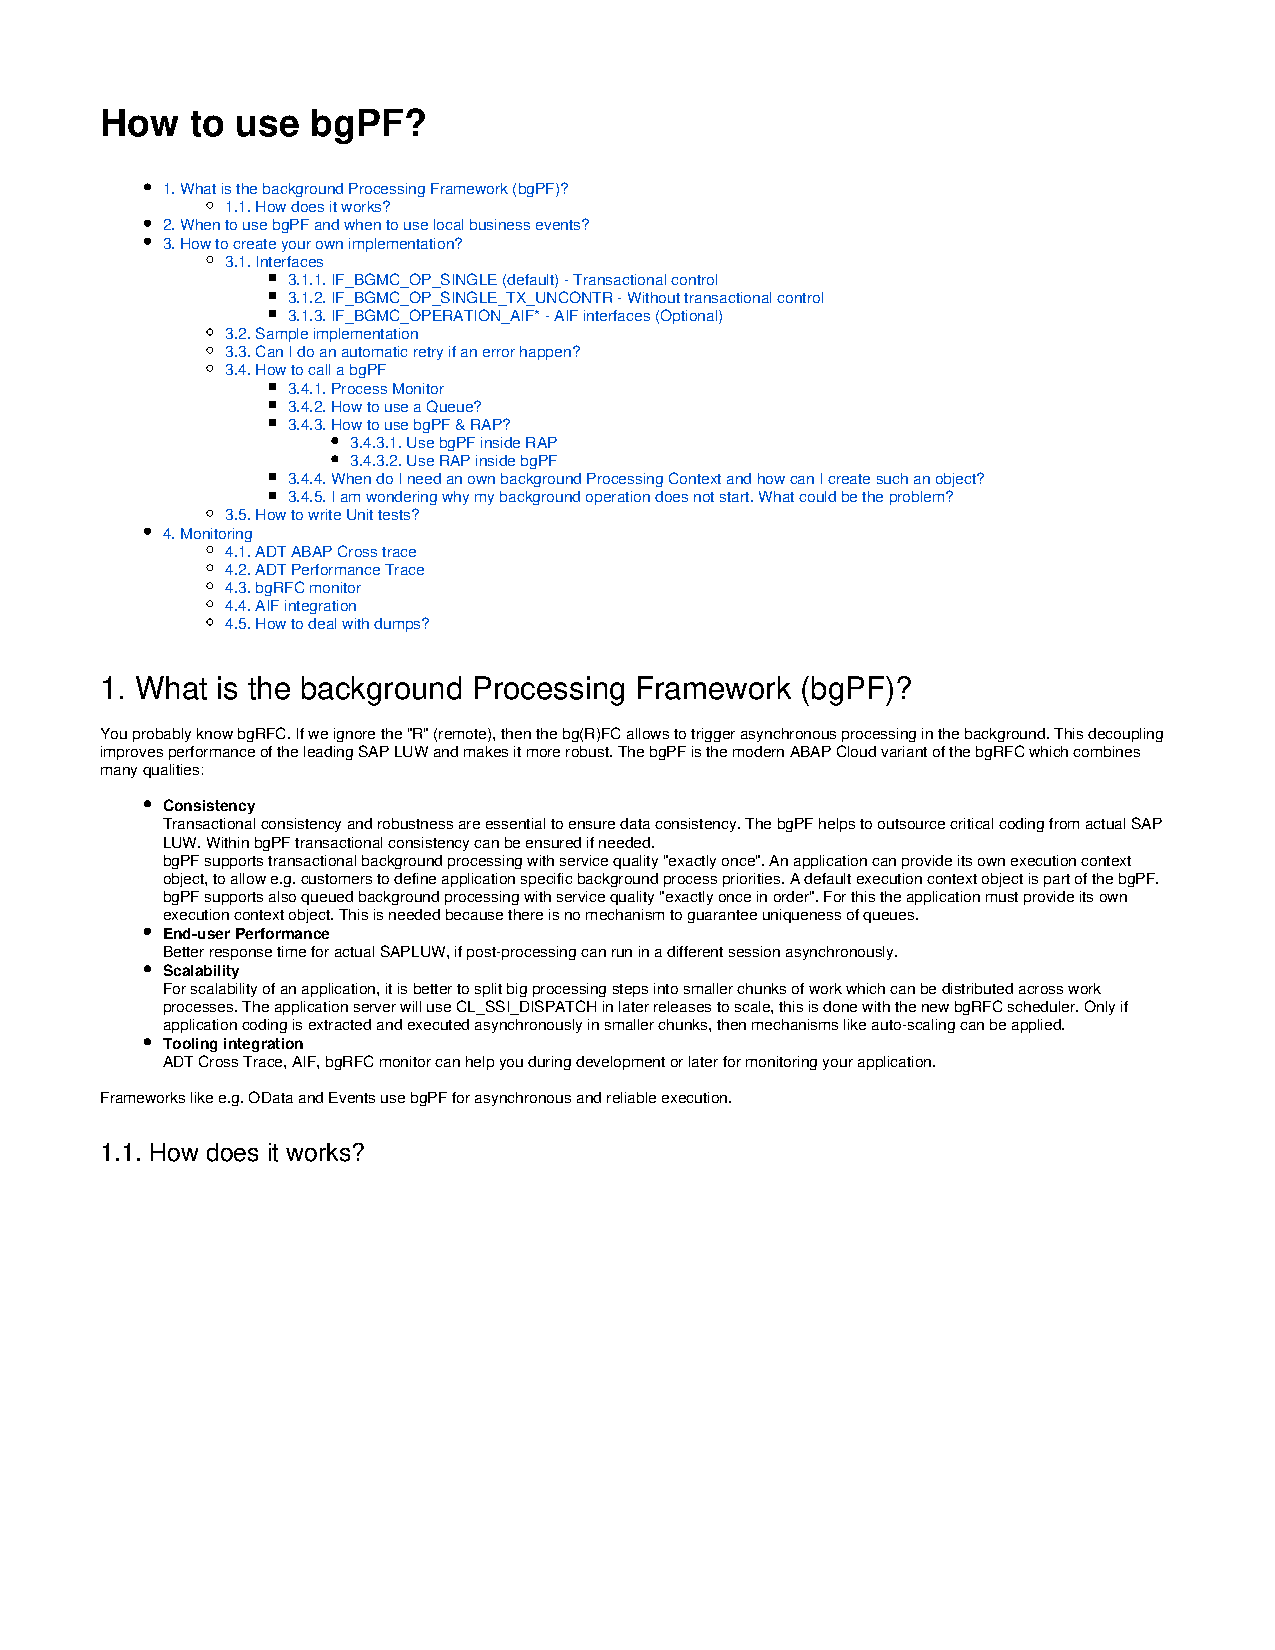
\includepdf[pages= 1, scale=0.8, pagecommand={}]{Literatur/bgPF_Wiki.pdf}
\end{figure}
\clearpage

\begin{figure}
    \includepdf[pages= 2, scale=0.8, pagecommand={}]{Literatur/bgPF_Wiki.pdf}
\end{figure}
\clearpage

\begin{figure}
    \includepdf[pages= 3, scale=0.8, pagecommand={}]{Literatur/bgPF_Wiki.pdf}
\end{figure}
\clearpage

\begin{figure}
    \includepdf[pages= 4, scale=0.8, pagecommand={}]{Literatur/bgPF_Wiki.pdf}
\end{figure}
\clearpage

\begin{figure}
    \includepdf[pages= 5, scale=0.8, pagecommand={}]{Literatur/bgPF_Wiki.pdf}
\end{figure}
\clearpage

\begin{figure}
    \includepdf[pages= 6, scale=0.8, pagecommand={}]{Literatur/bgPF_Wiki.pdf}
\end{figure}
\clearpage

\begin{figure}
    \includepdf[pages= 7, scale=0.8, pagecommand={}]{Literatur/bgPF_Wiki.pdf}
\end{figure}
\clearpage

\begin{figure}
    \includepdf[pages= 8, scale=0.8, pagecommand={}]{Literatur/bgPF_Wiki.pdf}
\end{figure}
\clearpage